
% ****************** Diaporama ******************
\documentclass{beamer}


% ****************** Packages ******************
\usepackage[french]{babel}
\usepackage[T1]{fontenc}
\usepackage[utf8]{inputenc}
\usepackage{tikz}
\usepackage{graphicx}
\usepackage{graphics}
\usepackage{caption}
\captionsetup[figure]{labelformat=empty} 

\usetheme{Warsaw}


% **** logo de l'upmc ****
\logo{
\includegraphics[width=2cm]{images/logo_upmc.png}}

\addtobeamertemplate{footline}{\insertframenumber/\inserttotalframenumber}

% ****************** Info pour page de garde ******************
\title{iBalezator}

\author{Adrien Ferreira, Alexandra Hospital}

\institute{PSAR - UPMC}

\date{16 avril 2015}



% ****************** Page de garde ******************
\begin{document}

   \begin{frame}

      \titlepage

   \end{frame}


% ******************** Table des matieres ********************
%  S'ajoute à chaque fin de section pour montrer 
%  où on est dans la présensation 

\AtBeginSection[]
{
\begin{frame}

     \frametitle{Sommaire}

        \tableofcontents[currentsection]

\end{frame} 
}


% ************ Présentation du projet ************ 

\section{Présentation du projet}

	% *** Balezator en ligne ***
	\subsection{Balezator en ligne}

	\begin{frame}

		\frametitle{Balezator en ligne}
			\begin{center}
				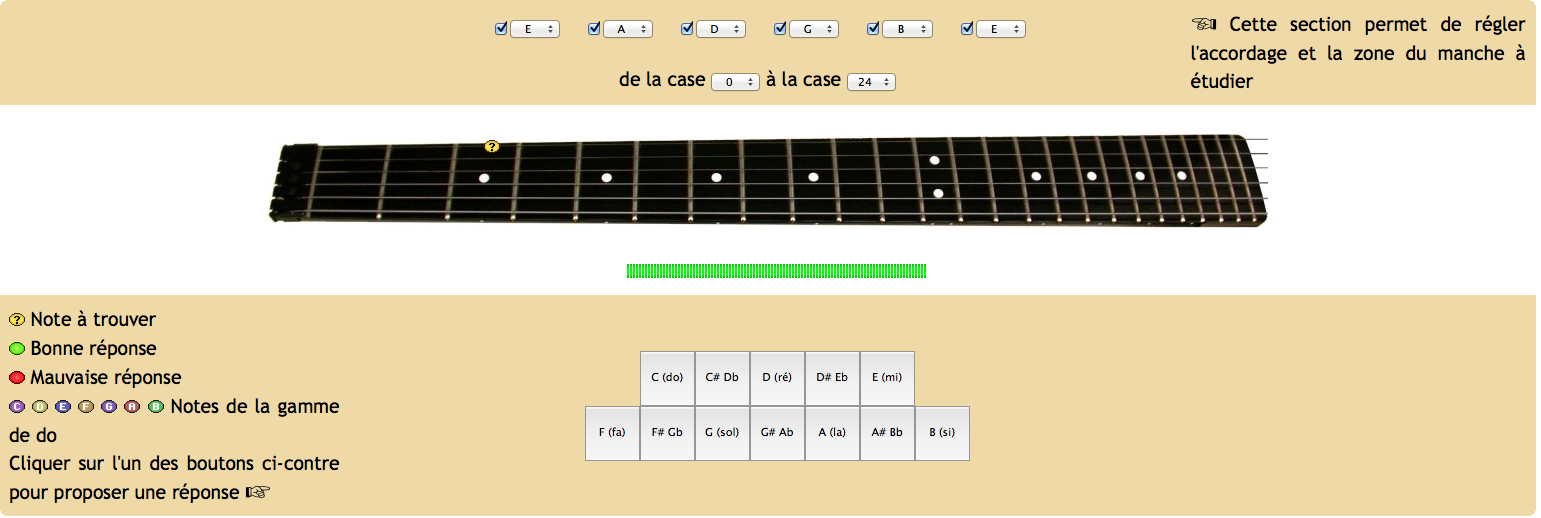
\includegraphics[width=8cm]{images/balezator_manche.png}
			\end{center}
			\begin{itemize}
				\item Jeu de devinettes pour apprendre la position des notes sur le manche
				\item Barre de score pour montrer la progression
			\end{itemize}
	\end{frame} 

	% *** iBalezator ***
	\subsection{iBalezator}
	\begin{frame}

		\frametitle{iBalezator}
		\begin{itemize}
			\item Adaptation du Balezator en ligne pour petits terminaux iOS 8.1
			\item Application dédiée aux guitaristes débutants
			\item Deux modes de jeu :
		\end{itemize}


		\begin{columns}

			 \begin{column}{0.5\textwidth}
				\begin{figure}
					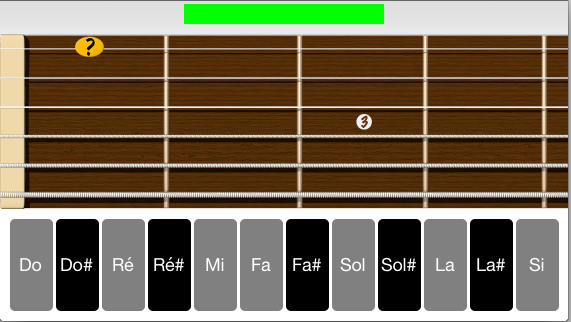
\includegraphics[width=5cm]{images/presentation_mc_question.png}
	
				\end{figure}

			\end{column}

			 \begin{column}{0.5\textwidth}
				\begin{figure}
					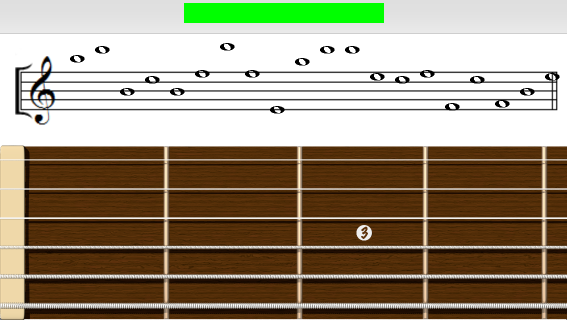
\includegraphics[width=5cm]{images/presentation_pm.png}
					
				\end{figure}
				
			\end{column}

		\end{columns} 
	\end{frame} 


% ******************* Le produit *******************
\section{Le produit}
	\begin{frame}

		\begin{itemize}
			\item Fusion des codes de maquettes et de fonctionnalités
			\item Architecture modifiée : MVC
			\item Amélioration de l'interface graphique
			\item Implémentation de fonctionnalités dans chaque mode
			\item Implémentation du changement de mode par glissement vertical
			\item Bibliothèque de son testée
		\end{itemize}

	\end{frame}



	\subsection{Mode manche/clavier}
		\begin{frame}
			\frametitle{Mode manche/clavier}

			\begin{minipage}{0.35\linewidth}
				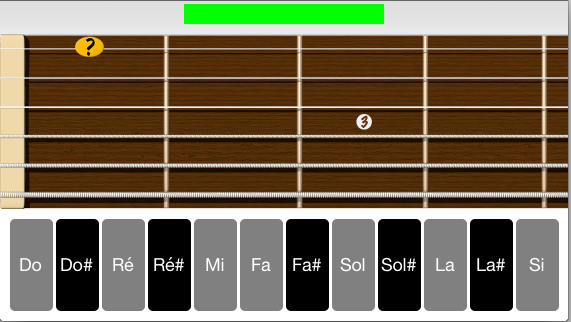
\includegraphics[width=4cm]{images/presentation_mc_question.png}
			\end{minipage}\hfill
			\begin{minipage}{0.6\linewidth}
				
				\begin{itemize}
					\item Tirage aléatoire d'une note sur tout le manche
					\item Affichage du marqueur de question
				\end{itemize}
			\end{minipage}
			\bigbreak

			\begin{minipage}{0.35\linewidth}
				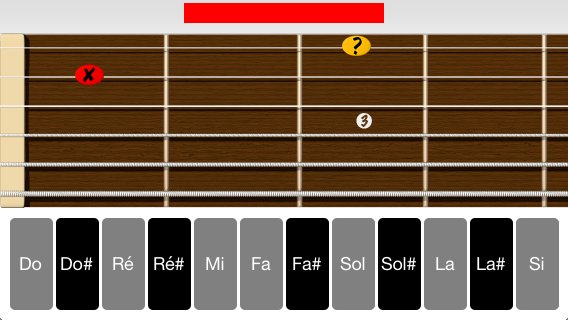
\includegraphics[width=4cm]{images/presentation_mc_bad.png}
			\end{minipage}\hfill
			\begin{minipage}{0.6\linewidth}
				\begin{itemize}
					\item Détection d'une mauvaise réponse
					\item Affichage de la fausse note sur le manche
					\item Mise à jour de la barre de score
				\end{itemize}
			\end{minipage}
			
		\end{frame}	

		\begin{frame}
			\frametitle{Mode manche/clavier}


			\begin{minipage}{0.35\linewidth}
				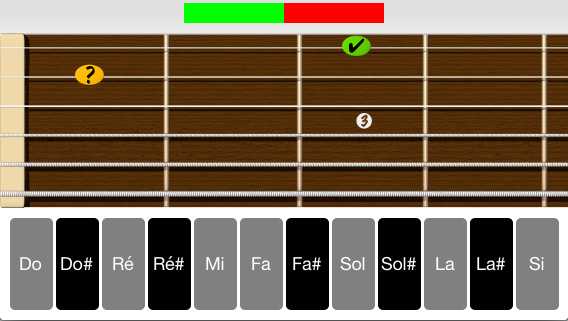
\includegraphics[width=4cm]{images/presentation_mc_good.png}
			\end{minipage}\hfill
			\begin{minipage}{0.6\linewidth}
				
				\begin{itemize}
					\item Détection d'une bonne réponse
					\item Affichage du marqueur de bonne réponse
					\item Génération d'une nouvelle note aléatoire
				\end{itemize}
			\end{minipage}
			\bigbreak

		\end{frame}	

	\subsection{Mode portée/manche}
		\begin{frame}
			\frametitle{Mode portée/manche}

			\begin{minipage}{0.35\linewidth}
				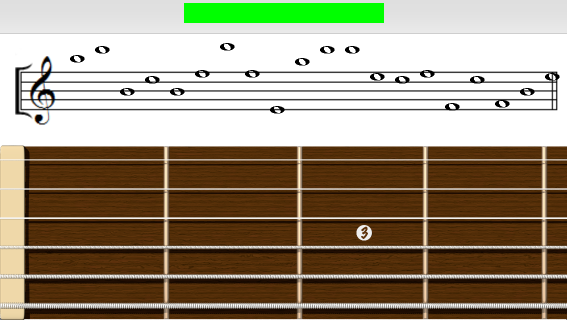
\includegraphics[width=4cm]{images/presentation_pm.png}
			\end{minipage}\hfill
			\begin{minipage}{0.6\linewidth}
				
				\begin{itemize}
					\item Génération de notes aléatoires
					\item Affichage sur la portée 
					\item Vérification de la note sur le manche
				\end{itemize}
			\end{minipage}
			
		\end{frame}	

%Bibliothèque de son


% ******************* Ce qu'il reste à faire *******************

\section{À implémenter}

	\begin{frame}
		\begin{itemize}
		\item Mode manche/clavier
			\begin{itemize}
				\item Temporisation
				\item Intégration du son
			\end{itemize}
		\item Mode portée/manche
			\begin{itemize}
				\item Temporisation
				\item Intégration du son
				\item Placement des notes
				\item Création du jeu
			\end{itemize}
		\end{itemize}

	\end{frame}



% ***** Implémentation *****

\section{Conclusion}

	\begin{frame}

	\begin{itemize}
		\item Organisation : des fonctionnalités basiques aux plus complexes
		\item Mode manche/clavier fonctionnel
		\item Mode portée/manche à continuer
		\item Questions :
			\begin{itemize}
				\item Mise à jour des vues ?
				\item Temporisation ? Utilisation de threads ?
			\end{itemize}
	\end{itemize}


	\end{frame}


\end{document}